
\section{Data}\label{Sec:Data}



%%%%%%%%%%%%%%%%%%%%%%%
%%%   Data source   %%%
%%%%%%%%%%%%%%%%%%%%%%%

\subsection{Source}\label{Sec:Data;Subsec:Source}

The data used for the present research was provided by Discovergy GmbH.\footnote{The data can be downloaded from \href{https://research.discovergy.com}{https://research.discovergy.com}.} Discovergy installs and maintains smart meters in German households for a one-time installation and monthly maintenance fee. Customers in return get various services centered around the analysis and visualization of their energy consumption and/or production. Discovergy describes itself as a full-range supplier of smart metering solutions offering transparent energy consumption and production data for private and commercial clients \citep{Discovergy:2018}. All energy measurements of their Discovergy smart meters can be accessed by customers through a web portal and mobile app. Additionally, various services are offered, such as, tips for energy savings potential, irregular consumption pattern warnings, personal energy reporting, and consumption analysis of individual appliances.

To be able to offer such data-driven services, Discovergy smart meters\footnote{Discovergy currently installs for private household clients the EasyMeter Q3D standard load profile meter which is connected to the Discovergy Meteorit TM smart meter gateway which records and transmits the recordings to Discovergy servers. The meter specifications can be found here: \texttt{https://discovergy.com/files/sources/product-information/SLP\_Zaehler.pdf} (in German).} record energy consumption and production near real-time -- i.e., 2-second intervals –- and send the readings to Discovergy's servers for storage and analysis. Therefore, Discovergy has extremely high resolution energy data of their customers at their disposal. This high resolution is in stark contrast to the half-hourly or even hourly recorded data used in previous studies \cite[e.g.,][]{Arora:2016,Auder:2018,Shi:2017,Gerossier:2017}.

To the authors knowledge, there is no research using Discovergy smart meter data, apart from \cite{Teixeira:2017} who used the data as simulation input but not for analysis or prediction. As Discovergy never provided data for external research purposes before, there was no suitable process to retrieve data from their internal data storage solutions available. For this reason, the author had to provide an API client for the Discovergy REST API to export data from pre-selected meters.


%%%%%%%%%%%%%%%%%%%%%%
%%%   Obtainment   %%%
%%%%%%%%%%%%%%%%%%%%%%

\subsection{Obtainment}\label{Sec:Data;Subsec:Obtainment}

As all Discovergy smart meters send their measurements in real-time to servers for storage, visualization and analysis, customers can access their meters and measurements through a web application and app. Additionally, customers with the need for automated data access can interact with the stored meter measurements through predefined endpoints. These endpoints serve as an application programming interface (API) called Discovergy REST API \citep{DiscovergyAPI:2018}. By providing the credentials for their Discovergy account\footnote{Sign up for a Discovergy account is open to everyone at https://my.discovergy.com/login. The account provides access to the Discovergy API for developers, without the need of being a Discovergy customer. However, only customers with an installed Discovergy smart meter, that is associated with their account, will have access to actual smart meter data. For testing purposes though, the Discovergy customer service can associate dummy meters as the one used for the demo web portal (\href{https://my.discovergy.com/dashboard?1}{https://my.discovergy.com/dashboard?1}) with any account.}, developers can send requests to a specified endpoint URL. The API returns to such a request a data object formatted in JavaScript Object Notation (JSON). For example, a user authenticates herself with her account credentials and requests the endpoint \texttt{/meters} with the verb \texttt{GET} at the base URL \texttt{https://api.discovergy.com/public/v1}. In response, the server returns a JSON object containing all meter IDs the user has access to.

To automate the process of data retrieval from the Discovergy servers, the author of this study had to program an API client, which is compliant with the constraints of a RESTful architecture.\footnote{REST refers to Representational State Transfer and describes an architetural style that ensures interoperability of systems through the web \cite[][Ch. 5]{fielding:2000}.} This client  had to be able to authenticate the user with account credentials provided in a flat file, request the readings for one year in 3-minute intervals of all meters specified in another flat file, and export the returned JSON data to a specified path. As the API had restrictions on the maximum time span of readings that could be returned depending on the measurement resolution (i.e., returns at most 10 days in 3-minute resolution), the client had to to make 37 request per meter to cover the whole year of 2017 in 10 day periods. As mentioned above, the measurement resolution of the Discovergy smart meters is with 2-second intervals much higher than the 3-minute intervals requested. However, the data management system employed by Discovergy already provides 3-minute aggregations of the original recordings which can be retrieved by specifying the according parameter in the API client.

The client was developed in Java based on the demo client provided in the Discovergy REST API documentation \citep{DiscovergyAPI:2018}. The code for the API client can be found in Appendix \ref{App:Code:C1API}. The client was sent to an Discovergy employee who used an administrative account with access to a sufficiently large number of smart meters to retrieve the data sets used in this study. Unfortunately, it is not known to the author what selection criteria, other than having complete data for all of 2017, where used by Discovergy internally to chose the meters of which the data was provided. Therefore, it is not possible to evaluate how representative the provided data is regarding Discovergy customers or even energy consuming/producing household in general.
After retrieving the data, Discovergy converted the data to csv-files. To facilitate the file transfer, the resulting files were made available online and can by now be downloaded by the general public here: \href{https://research.discovergy.com}{https://research.discovergy.com}. 



%%%%%%%%%%%%%%%%%%%%%%%%%%%%
%%%   Data description   %%%
%%%%%%%%%%%%%%%%%%%%%%%%%%%%

\subsection{Description}\label{Sec:Data;Subsec:Description}

The data comes in 200 individual csv-files each containing the meter readings of a single smart meter. The readings are recorded in 3-minute intervals and range from 01.01.2017 00:00:00 to 01.01.2018 00:00:00. This translates into 175,201 observations per smart meter. Each smart meter measures energy consumption,  energy production and power over all phases installed in the meter and records them together with a timestamp in Unix milliseconds. For this research, only energy consumption and production are relevant. In summary, the data used here are 200 individual data sets each containing two time series (energy consumption and energy production) with 175,201 observations evenly spaced in 3-minute intervals.

Below, a preprocessed and correctly formatted sample of the data for consumer 56 and prosumer 89 containing 6 measurement points are shown.

\begin{table}[ht]
    \csvreader[centered tabular=c|cc,
    table head=
    \hline\hline
    \textbf{time} & \textbf{energy} & \textbf{energyOut} \\
    \hline
    \ldots & \ldots & \ldots \\,
    head to column names,
    separator=comma,
    respect all,
    late after line=\\,
    table foot=
    \ldots &  \ldots & \ldots \\\hline\hline]
    {tables/consumer-00000056_glimpse.csv}{}%
    {\csvcolii & \csvcoliii & \csvcoliv}%
    \caption[Data excerpt of consumer 056]{Data excerpt of consumer 056. \quantnet}
    \label{Tab:c056}
\end{table}

\begin{table}[ht]
    \csvreader[centered tabular=c|cc,
    table head=
    \hline\hline
    \textbf{time} & \textbf{energy} & \textbf{energyOut} \\
    \hline
    \ldots & \ldots & \ldots \\,
    head to column names,
    separator = comma,
    respect all,
    late after line = \\,
    table foot = \ldots & \ldots & \ldots \\\hline\hline]
    {tables/producer-00000089_glimpse.csv}{}%
    {\csvcolii & \csvcoliii & \csvcoliv}%
    \caption[Data excerpt of prosumer 089]{Data excerpt of consumer 089. \quantnet}
    \label{Tab:p089}
\end{table}

The energy and energy out readings are recorded in the unit $10^{-10}$ kWh. \texttt{energy} records the meter's energy consumption reading at time $t$ (e.g., in Table \ref{Tab:c056}, since the meter installation and up until 2017-09-20 12:18:00, consumer 056 consumed \csvreader[
filter equal = {\thecsvinputline}{2}]%
{tables/consumer-00000056_glimpse.csv}{}%
{\csvcoliii}$\times 10^{-10}$ kWh). \texttt{energyOut} records the meter's energy production reading (e.g., in Table \ref{Tab:p089}, since the meter installation and up until 2017-09-20 12:18:00, prosumer 089 fed into the grid \csvreader[
filter equal = {\thecsvinputline}{2}]%
{tables/producer-00000089_glimpse.csv}{}%
{\csvcoliii}$\times 10^{-10}$kWh). As consumer 056 is not a prosumer and has no energy production capacity installed, all energy out readings must be zero. Note, however, that although the data excerpt of prosumer 089 shown here has positive energy out readings, there may be prosumers with all zero energy out readings if their production capacity never exceeds their own consumption. In this case, the prosumer never actually feeds energy into the grid and the meter records an energy out reading of zero at all measurement points.

For further computations, the first-order differences of the energy consumption and production readings were calculated. These first-order differences are equivalent to the energy consumption/production within each 3-minute interval between two meter recordings. The result of this computation leaves each time series with 175,200 observations.\footnote{One regular year (no leap year) comprises 175,200 3-minute intervals: $365\text{d} * 24\text{h/d} * \frac{60\text{m/h}}{3\text{m}} = 175,200$.}



%%%%%%%%%%%
\subsubsection{Consumer data sets}

Figure \ref{Fig:energycons_c082} exemplary shows the energy consumption time series of consumer 082. It will be discussed here to gain a better understanding of the data at hand. For easier readability, the unit of consumption has been converted from $10^{-10}$ kWh to kWh. In the first panel of Figure \ref{Fig:energycons_c082}, the consumption per 3-minute interval for all of 2017 is shown. The consumption per 3-minute interval fluctuates between 0 and 0.361 kWh with a mean of 0.039 kWh and a median of 0.024 kWh.\footnote{For comparison, an average German single household consumes 2300 kWh per year. This is equivalent to 0.013 kWh per 3-minute interval. Hence, it is reasonable to assume that consumer 082 is a multi-person household.}

Notably, there are two extended (in March and June) and three shorter periods (in July, September, and December) of clearly distinguishable low consumption and low fluctuation levels. The most likely explanations for these low, stable energy consumption periods are holidays, in which the household members are on vacation and leave appliances that are on standby or always turned on as the only energy consumers. This exemplifies the fact, that household members' behaviour is the biggest driver of fluctuations in the energy consumption of a household and the almost only cause for uncertainty in the time series.

Interestingly, the consumption time series of consumer 082 shows an increase in mean consumption starting with October 2017. This could be explained by colder outside temperatures. However, within the first quarter of 2017, no equivalent decrease in the mean energy consumption can be seen. Therefore, the reason for this increase might be given by newly acquired household appliances which are increasingly used with the approaching winter as the household members spend more time indoors.

\begin{figure}[ht]
 \centering
\includegraphics[width=\textwidth]{thesis/graphs/timeseries/c082_cons.pdf}
\caption[Energy consumption recordings for consumer 082]{Energy consumption recordings for consumer 082. The first panel shows the full year 2017, the second panel zooms in to one month (May), and the third panel zooms in to one day (May, 13). \quantnet}
\label{Fig:energycons_c082}
\end{figure}

The second panel zooms to just one month making daily fluctuation patterns already visible. In May there seem to be no abnormal consumption patterns. There are a few peaks in the first and third week of May that stand out, but no longer periods of very low energy consumption. More interestingly seems to be the last panel, which zooms in to just one day of energy consumption, i.e. May 13, 2017. This day was chosen for no particular reason other than that it is more or less in the middle of the month shown in the second panel. May 13, however, nicely exemplifies a usual pattern of energy consumption: There is low and rather stable energy consumption from midnight until about 7.30 a.m. which only fluctuates in a systematic and repeated way. Most probably, this "base" consumption is caused by appliances in standby and "always on" appliances, such as a fridge and/or freezer. At around 7.30 a.m., the household members probably wake up and the energy consumption spikes for the next 30 minutes -- the light is turned on, coffee is made, the stove is turned on, and maybe a flow heater is used to shower with hot water. As the household members leave the house (May 13 is a Monday), the consumption slowly decreases again. In the evening at about 6.30 p.m. energy consumption spikes again, probably caused by dinner preparations (and the usage of a microwave or stove). Not intuitively explainable, however, is the spike which is visible just before midnight. This spike, again, highlights the extreme uncertainty contained in individual household energy consumption. It is mostly caused by human behavior, which can seem quite erratic by just looking at energy consumption patterns without context.

To get a better impression of the representativity of consumer 082's  energy consumption, it is compared to the other data sets available for this study. Figure \ref{Fig:total_consumption} shows the total energy consumption of all consumers in kWh for 2017. As can be seen, consumer 082 (labelled c082 in Figure \ref{Fig:total_consumption}) is at the lower end of the top quartile of the total energy consumption distribution across all consumers. The household's total energy consumption in 2017 was 6752.763 kWh. According to \citet{Stromspiegel:2017}, this number corresponds to a category D five-person household (on a scale from A (very low) to G (very high energy consumption)) that is heating its water with electricity. That means, the household of consumer 082 is either very big or has a comparatively very high energy consumption. Consumer 067, on the contrary, is remarkable as total consumption here is with only 40 kWh quite close to zero. At the high end of total consumption is consumers 025 with almost five times the total consumption of the average consumer in this data sets. Summary statistics for the total energy consumption of consumer households in 2017 can be found in Appendix \ref{App:Tables:totalcons}.

\begin{figure}[ht]
 \centering
\includegraphics[width=\textwidth]{thesis/graphs/consumer_totalconsumption.pdf}
\caption[Consumers' total energy consumption (in kWh) in 2017 ordered from high to low]{Consumers' total energy consumption (in kWh) in 2017 ordered from high to low. \quantnet}
\label{Fig:total_consumption}
\end{figure}

Figure \ref{Fig:boxplots_consumption} offers another view on the consumers' energy consumption. The figure shows a boxplot for each consumer's distribution of energy consumption per 3- minute interval. That means, the median line in the boxplot of a consumer is the consumers median consumption per 3-minute interval, while the box encloses the interquartile range (IQR) of the 3-minute consumption values of this particular consumer. It is apparent, that the IQR is for almost all consumers relatively small compared to the total range of their consumption values. All points plotted above the boxplots' whiskers are consumption values greater than the third quartile plus 1.5 $\times$ IQR. This again shows that there is a substantial amount of extreme values -- for which the description "outlier" not necessarily fits as they obviously occur quite often -- which are hard to predict with standard forecasting methods.

\begin{figure}[ht]
 \centering
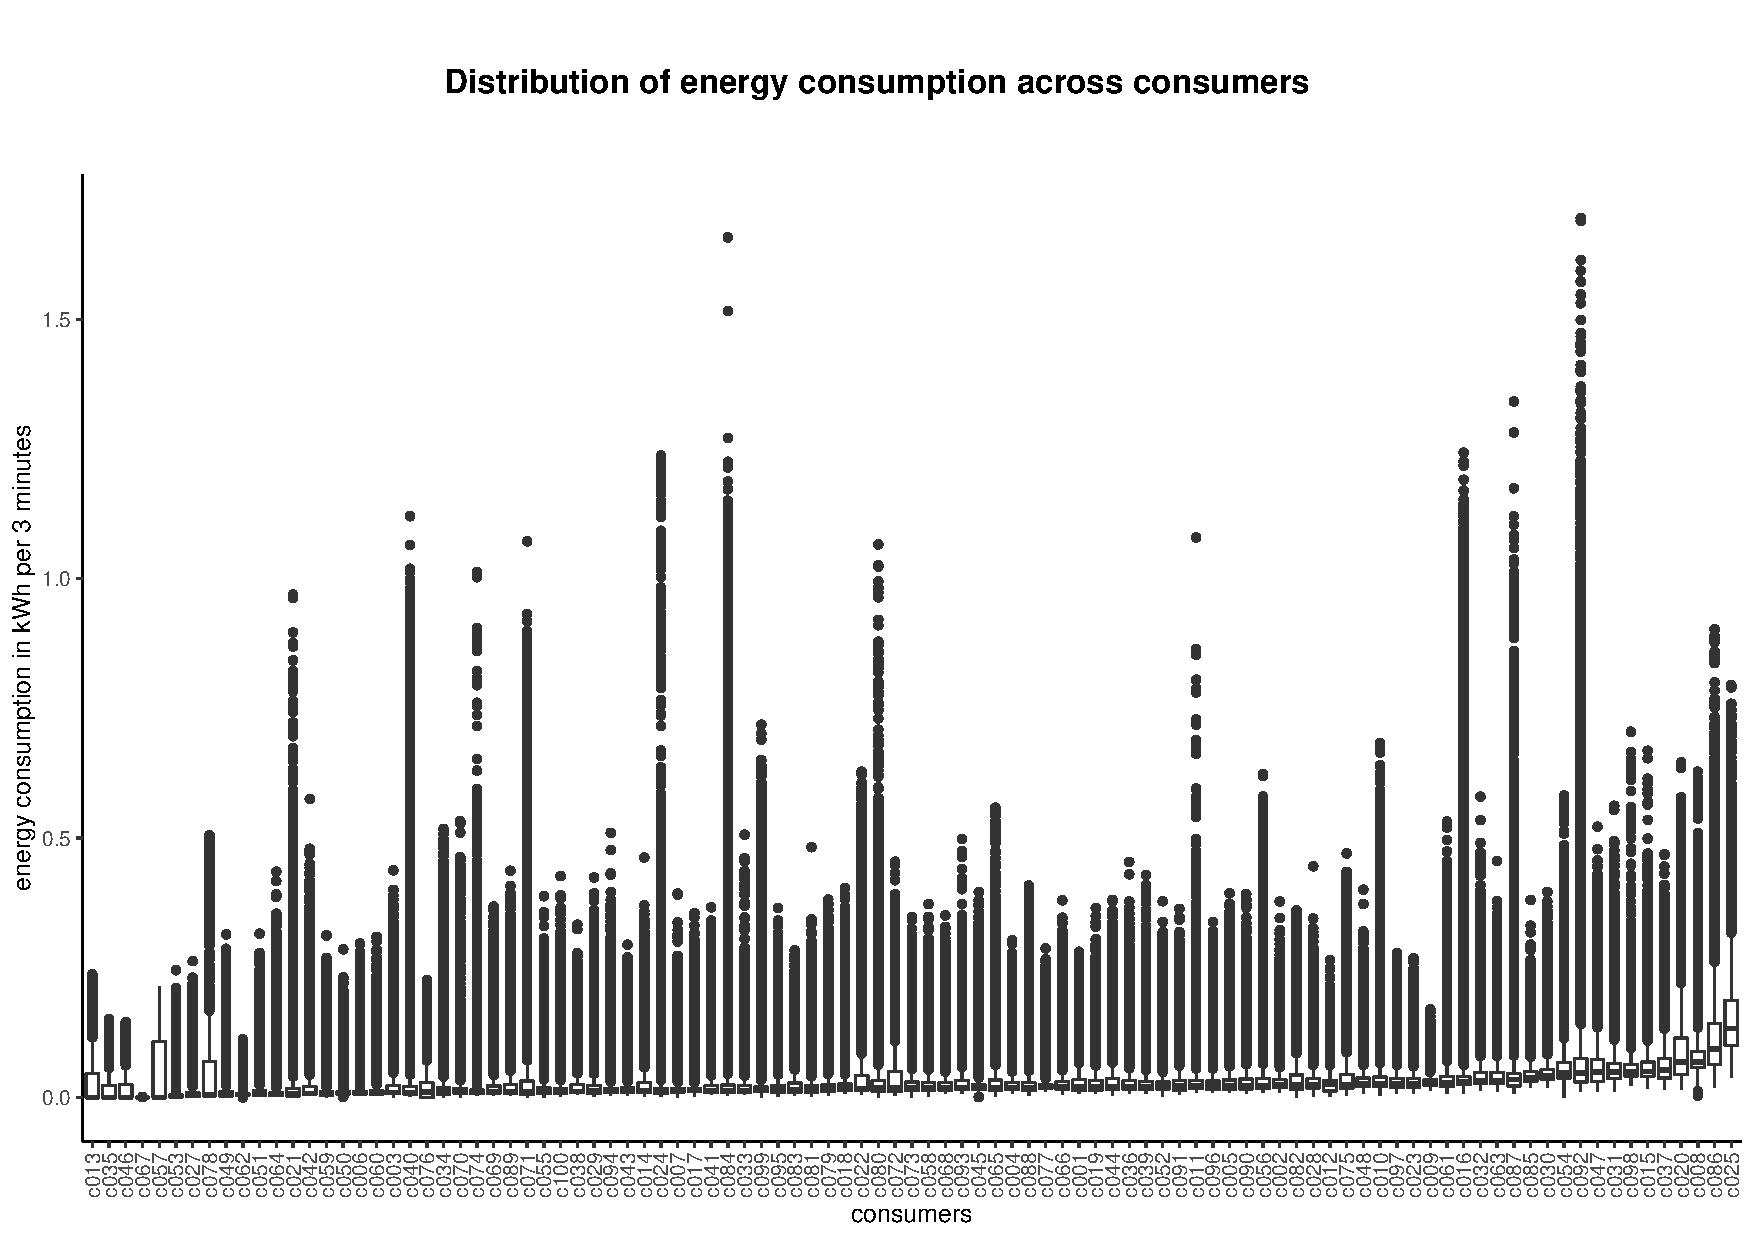
\includegraphics[width=\textwidth]{thesis/graphs/consumer_boxplots_consumption.jpg}
\caption[xxx]{xxx. \quantnet}
\label{Fig:boxplots_consumption}
\end{figure}

%%%%%%%%%%%
\subsubsection{Prosumer data sets}

The prosumer data sets show partially very different consumption patterns than pure consumers. This due to the fact, that the recorded energy consumption per 3-minute interval is the net value of the actual energy consumption and the energy production in the same interval. For example, if prosumer 024's recorded consumption value is 0.021 kWh in the time period from 2017-05-13 06:03:00 to 06:06:00, and its energy production in the same interval is 0.018 kWh (which is not recorded and therefore not known), its actual energy consumption in that time interval is 0.039 kWh. However, this actual energy consumption is unknown as the energy production per 3-minute interval is not recorded. Only a surplus of energy production over consumption would be recorded as an increase in the energy out readings (see Table \ref{Tab:p089}) -- which is not the case in this example.

Moreover, the total consumption in 2017 of prosumers is very 

\begin{figure}[ht]
 \centering
\includegraphics[width=\textwidth]{thesis/graphs/timeseries/p0xx_cons.pdf}
\caption[Energy consumption recordings for prosumer 0xx]{Energy consumption recordings for prosumer 0xx. The first panel shows the full year 2017, the second panel zooms in to one month (May), and the third panel zooms in to one day (May, 13). \quantnet}
\label{Fig:energycons_p0xx}
\end{figure}



%%%%%%%%%%%%%%%%%%%%%%%%%%%%%%
%%%   Data sets excluded   %%%
%%%%%%%%%%%%%%%%%%%%%%%%%%%%%%

\subsection{Peculiarities in the data}

The data sets were analyzed for peculiarities the time series patterns that seemed to be systematically different than the majority of data sets. One such peculiarity is the occurrence of zero values. In any household that does not produce its own energy (pure consumer household), energy consumption of 0 kWh, even only for a very short period of time, seems to be very unlikely (apart from the rare case of a power outage in the area or when the main switch of the household is turned off). Thus, it is not surprising that 93 \% of the data sets do not contain any 0 kWh measurements per 3-minute interval at all. Of the remaining 6 data sets, one contains just a single measurement of 0 kWh, which seems plausible. The other data set with a negligible amount of zero values is consumer 082 which was discussed in detail in section \ref{Sec:Data;Subsec:Description}. In Figure \ref{Fig:energycons_c082}, it is visible that although the consumption pattern does not change substantially, the lowest values of the daily fluctuations are lower in the second half of 2017 than in the first half. However, this seems still a plausible consumption pattern for a typical household. The other five data sets, however, contain between 34 and 54 \% of zero values. Examining the consumption time series more closely also reveals, that these households exhibit a systematically different consumption pattern that one would expect from a typical household.

\begin{sidewaysfigure}[htbp]
    \centering
    \begin{minipage}[ht]{\dimexpr.5\textheight-0.15em}
    \includegraphics[width=\textwidth]{thesis/graphs/timeseries/c013_cons.pdf}
    \end{minipage}
    \begin{minipage}[ht]{\dimexpr.5\textheight-0.15em}
    \includegraphics[width=\textwidth]{thesis/graphs/timeseries/c035_cons.pdf}
    \end{minipage}\\
    
    \begin{minipage}[ht]{\dimexpr.5\textheight-0.15em}
    \includegraphics[width=\textwidth]{thesis/graphs/timeseries/c067_cons.pdf}
    \end{minipage}
    \begin{minipage}[ht]{\dimexpr.5\textheight-0.15em}
    \includegraphics[width=\textwidth]{thesis/graphs/timeseries/c076_cons.pdf}
    \end{minipage}
    \caption[Energy consumption recordings for consumer with conspicuous consumption patterns]{Energy consumption recordings for consumer with conspicuous consumption patterns.}
    \label{fig:energycons_peculiar}
\end{sidewaysfigure}

Figure \ref{fig:energycons_peculiar} shows the time series of the aforementioned four consumers with a high share of zero measurements. Consumer 013 and 035 both show a very similar pattern of daily energy consumption. Looking at the middle panel of the two upper graphs in Figure \ref{fig:energycons_peculiar}, the regularity of the consumption increases and decreases for each day is striking. The lower panel shows again, exemplary May 13. Energy consumption starts to almost linearly increasing at about 6 a.m. and decreases to 0 kWh at about 6 p.m. This also explains the 52.77 and 54.02 \% of zero values in those to data sets: almost exactly 12 hours per day (from midnight to 6 a.m. and from 6 p.m. to midnight) the consumption is zero, while it is positive in between. and  In the meantime the the energy consumption fluctuates but with a relatively high "base" consumption. Switching back to the middle panel, it is noticeable that there are some days in May with an even smoother energy consumption increase and decrease over the course of the day. As there is no further socio-demographic data available, we can only guess what the reason for such different consumption patterns are. The most likely explanation seems to be, that the consumption time series of consumer 013 and 035 belongs to a small business rather than to a household.

The lower two graphs show the energy consumption time series of consumer 067 and consumer 075. Consumer 067 consumption pattern zoomed in to one month (middle panel) rather looks like an electrocardiogram (ECG) than what one would expect from a household energy consumption time series. The regularity of amplitude and frequency is obvious but not easily explained. Consumers 076 consumption pattern looks less suspicious at first sight. However, closer inspection reveals the same daily pattern of increasing consumption throughout the day and very low to zero energy consumption at night. This again rather resembles the energy consumption pattern of a business building or office rooms.



%%%%%%%%%%%
\subsubsection{Consumer data sets}



%%%%%%%%%%%
\subsubsection{Prosumer data sets}

%%%%%%%%%%%%%%%%%%%%%%%%%%%%%%%%%%%%%%%%%%%%%%%%%%%%%%%%%%%%%%%%%

\begin{itemize}

    \item Describe the data and its quality.
    \item How was the data sample selected?
    \item Provide descriptive statistics such as:
        \begin{itemize}
            \item time period,
            \item number of observations, data frequency,
            \item mean, median,
            \item min, max, standard deviation,
            \item skewness, kurtosis, Jarque--Bera statistic,
            \item time series plots, histogram.
        \end{itemize}
    \item For example:
        \begin{table}[ht]

        \begin{center}
            {\footnotesize
            \begin{tabular}{l|cccccccccc}
                \hline \hline
                           & 3m    & 6m    & 1yr   & 2yr   & 3yr   & 5yr   & 7yr   & 10yr  & 12yr  & 15yr   \\
                \hline
                    Mean   & 3.138 & 3.191 & 3.307 & 3.544 & 3.756 & 4.093 & 4.354 & 4.621 & 4.741 & 4.878  \\
                    StD    & 0.915 & 0.919 & 0.935 & 0.910 & 0.876 & 0.825 & 0.803 & 0.776 & 0.768 & 0.762  \\
                \hline \hline
            \end{tabular}}
        \end{center}
        \caption{Some descriptive statistics of location and dispersion for
        2100 observed swap rates for the period from February 15, 1999
        to March 2, 2007. Swap rates measured as 3.12 (instead of 0.0312). See Table
        \ref{Tab:DescripStatsRawDataDetail} in the appendix for
        more details.}
        \label{Tab:DescripStatsRawData}
        \end{table}

    \item Allows the reader to judge whether the sample is biased or to evaluate possible impacts of outliers, for
    example.

\end{itemize}
